% document style header
\documentclass[a4paper, 12pt]{config/homework}

% import default packages
\usepackage{config/packages}
\usepackage{config/commands}

% end preamble
\begin{document}

% document title
\noindent
Calvin Sprouse \hfill PHYS475 Homework 6 \hfill 2024 May 20
\bigskip

% homework problems begin
\begin{enumerate}
\item Use
\[\vec{B}_\text{int} = \frac{1}{4\pi \epsilon_0} \frac{e}{m_e c^2 r^3} \vec{L},\]
where \(e\) is the elementary charge, to estimate the internal magnetic field in a hydrogen atom. This value characterizes the boundary between the strong and weak field limit.

\bigskip
The magnitude of the internal magnetic field is given by
\[\vec{B}_\text{int}\cdot\vec{B}_\text{int}
= \left|\vec{B}_\text{int}\right|
= \left(\frac{1}{4\pi\epsilon_0}\frac{e}{m_e c^2}\right)^2\left(\frac{1}{r^3}\right)^2 \left|\vec{L}^2\right|.\]
Let \(\beta\) be defined as the pre-factors,
\[\beta \equiv \frac{1}{4\pi\epsilon_0}\frac{e}{m_e c^2}.\]
Then, the magnitude of the internal magnetic field may be represented in terms of operators
\[\left|\vec{B}_\text{int}\right|
= \hat{B}_\text{int} = \beta^2\frac{1}{\hat{r}^3}\frac{1}{\hat{r}^3}\hat{L}^2.\]
The average internal magnetic field can then be found as
\[\bra*{\Psi}\hat{B}_\text{int}\ket*{\Psi}
= \beta^2\bra*{\Psi}\left(\frac{1}{\hat{r}^3}\frac{1}{\hat{r}^3}\hat{L}^2\right)\ket*{\Psi} = \beta^2 \expval{\frac{1}{r^3}\frac{1}{r^3}L^2}.\]
We may insert the identity matrix between each of the three terms of the expectation value. The identity matrix may be expressed as the outer-product of wavefunctions. This allows us to express the expectation value of the internal magnetic field as
\[\expval{B_\text{int}} = \beta^2\expval{\frac{1}{r^3}}\expval{\frac{1}{r^3}}\expval{L^2}.\]
These expectation values are known for our chosen basis:
\[\expval{\frac{1}{r^3}} = \frac{1}{l\left(1+\frac{1}{2}\right)(l+1)n^3a^3}, \quad
\expval{L^2} = \hbar^2l(l+1).\]
Then,
\[\expval{B_\text{int}} = \beta^2\frac{\hbar^2l(l+1)}{\left[l\left(l+\frac{1}{2}\right)(l+1)n^3a^3\right]^2} = \beta^2 \frac{\hbar^2}{l(l+1)\left[\left(l+\frac{1}{2}\right)n^3a^3\right]^2}.\]
This implies that the strength of the internal magnetic field is strongest at low values of \(n\) and \(l\), which makes sense by the classical picture. Let \(n=1\). Then, \(l\in\left\{0, 1\right\}\). While \(l=0\) appears problematic, we recall that for \(l=0\) \(\expval{L^2}=0\) and thus \(\expval{B_\text{int}}=0\). Therefore, let \(l=1\). Then, substituting known values,
\[\expval{B_\text{int}} \approx \qty{34}{\tesla}.\]
Therefore, \(\left|B_\text{ext}\right|\ll \qty{30}{\tesla}\) is a weak field while \(\left|B_\text{ext}\right| \gg \qty{30}{\tesla}\) is a strong field.


\pagebreak
\item Consider the eight \(n=2\) states for the hydrogen atom, \(\bra*{2, l, j, m_j}\). Determine the energy of each state under weak-field Zeeman splitting and construct a diagram like the one in Figure 6.11 of Griffiths to show how the energies evolve as a function of \(B_\text{ext}\). Label each line clearly and indicate the slope of each line on the graph.

The total energy of each of the eight states is given by the sum of Equation~7.69, the Bohr energy and fine-structure correction, and Equation~7.79, the Zeeman effect energy. Equation~7.79 expresses the Zeeman effect energy as
\[E_Z^1 = \mu_B B_\text{ext} g_J m_j.\]
The Land\'{e} g-factor, \(g_J\), is given as part of Equation~7.78 as
\[g_J = \left(1 + \frac{j(j+1)-\ell(\ell+1)+s(s+1)}{2j(j+1)}\right).\]
For electrons, \(s=1/2\). Then, the Land\'{e} g-factor may be computed and multiplied by the allowed values of \(m_j\) for all eight states.
\begin{table}[h]
\centering
\begin{tabular}{c|cccc|cc}
\(\ket*{\Psi}\) & \(n\) & \(\ell\) & \(j\) & \(m_j\) & \(g_J\) & \(E_Z^1\)                           \\ \hline
\(\ket*{1}\)    & 2     & 0        & 1/2   & 1/2     & 2       & \(\mu_B B_\text{ext}\)              \\
\(\ket*{2}\)    & 2     & 0        & 1/2   & -1/2    & 2       & \(-\mu_B B_\text{ext}\)             \\
\(\ket*{3}\)    & 2     & 1        & 1/2   & 1/2     & 2/3     & \(\frac{1}{3}\mu_B B_\text{ext}\)   \\
\(\ket*{4}\)    & 2     & 1        & 1/2   & -1/2    & 2/3     & \(-\frac{1}{3}\mu_B B_\text{ext}\)  \\
\(\ket*{5}\)    & 2     & 1        & 3/2   & 3/2     & 4/3     & \(2 \mu_B B_\text{ext}\)            \\
\(\ket*{6}\)    & 2     & 1        & 3/2   & 1/2     & 4/3     & \(\frac{2}{3} \mu_B B_\text{ext}\)  \\
\(\ket*{7}\)    & 2     & 1        & 3/2   & -1/2    & 4/3     & \(-\frac{2}{3} \mu_B B_\text{ext}\) \\
\(\ket*{8}\)    & 2     & 1        & 3/2   & -3/2    & 4/3     & \(-2\mu_B B_\text{ext}\)
\end{tabular}
\end{table}

\pagebreak
For plotting purposes, we are interested in the factor in front of \(\mu_B B_\text{ext}\), the slope. Then, the quantities needed for plotting are given by the table below.
\begin{table}[h]
\centering
\begin{tabular}{c|ccc}
\(\ket*{\Psi}\) & \(j\) & \(\frac{E_Z^1}{\mu_B B_\text{ext}}\) & \(E_{nj}\)                                                        \\ \hline
\(\ket*{1}\) & 1/2 & \(\phantom{-}1\) & \(-\frac{\qty{13.6}{\eV}}{4}\left[1+\frac{5}{16}\alpha^2\right]\) \\
\(\ket*{2}\) & 1/2 & \(-1\) & \(-\frac{\qty{13.6}{\eV}}{4}\left[1+\frac{5}{16}\alpha^2\right]\) \\
\(\ket*{3}\) & 1/2 & \(\phantom{-}\frac{1}{3}\) & \(-\frac{\qty{13.6}{\eV}}{4}\left[1+\frac{5}{16}\alpha^2\right]\) \\
\(\ket*{4}\) & 1/2 & \(-\frac{1}{3}\) & \(-\frac{\qty{13.6}{\eV}}{4}\left[1+\frac{5}{16}\alpha^2\right]\) \\
\(\ket*{5}\) & 3/2 & \(\phantom{-}2\) & \(-\frac{\qty{13.6}{\eV}}{4}\left[1+\frac{1}{16}\alpha^2\right]\) \\
\(\ket*{6}\) & 3/2 & \(\phantom{-}\frac{2}{3}\) & \(-\frac{\qty{13.6}{\eV}}{4}\left[1+\frac{1}{16}\alpha^2\right]\) \\
\(\ket*{7}\) & 3/2 & \(-\frac{2}{3}\) & \(-\frac{\qty{13.6}{\eV}}{4}\left[1+\frac{1}{16}\alpha^2\right]\) \\
\(\ket*{8}\) & 3/2 & \(-2\) & \(-\frac{\qty{13.6}{\eV}}{4}\left[1+\frac{1}{16}\alpha^2\right]\)
\end{tabular}
\end{table}

\begin{figure}[H]
\centering
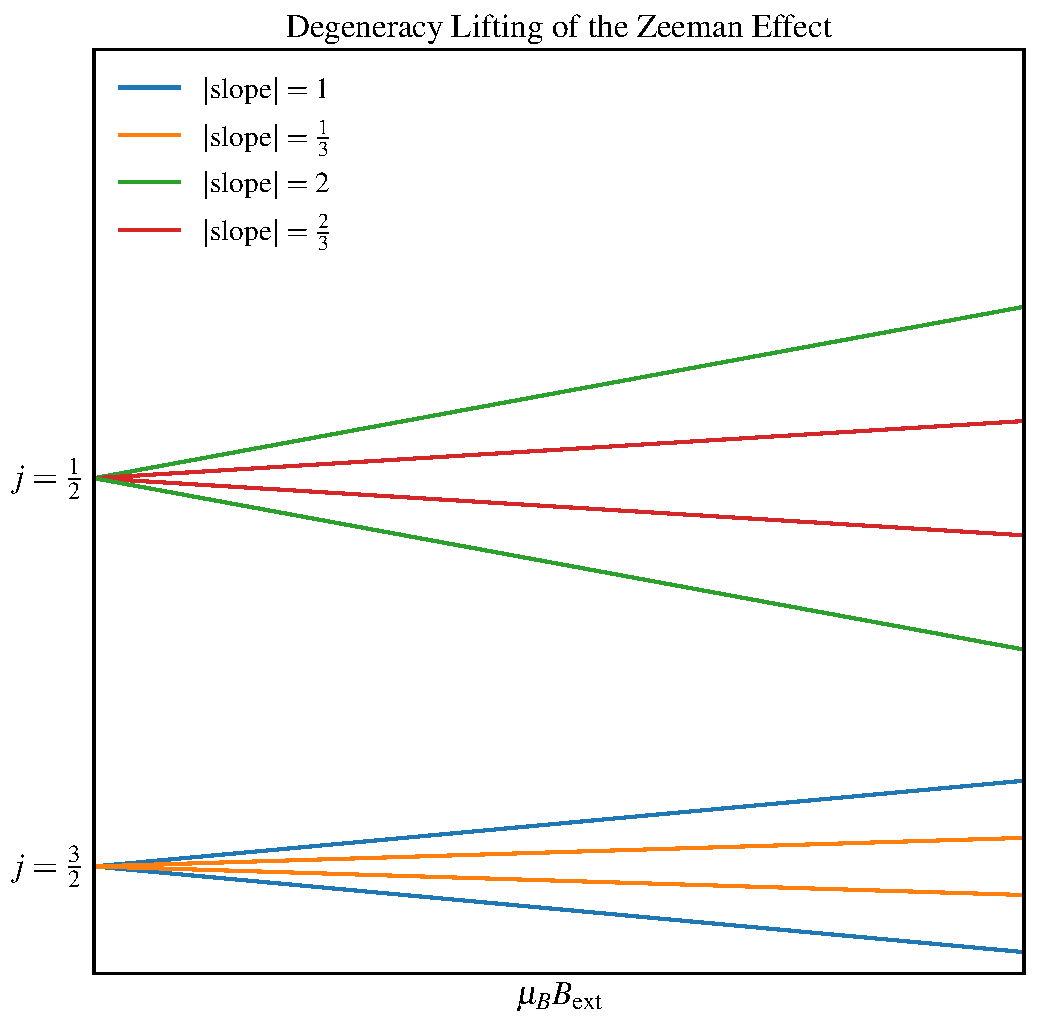
\includegraphics[width=0.7\textwidth]{notebooks/figures/energy_degeneracy_lifting.pdf}
\caption{The degeneracy lifting of the \(n=2\) state by the Zeeman effect. The colored lines represent the magnitude of the slope which is given by \(g_Jm_j\).}
\label{fig:degen}
\end{figure}

\end{enumerate}
\end{document}
